%% Signale.tex
%% $Id: Signale.tex 4 2005-10-10 20:51:21Z bless $
%%

Das Kapitel \textbf{Implementierung} wird anhand dem im Entwurf besprochenen Verlauf der Studie erkl{\"a}rt.

Bei der Entwicklung des Programms hat man sich Gedanken {\"u}ber ein System gemacht, bei dem man alle Daten schon digital abgespeichert hat und nicht noch Informationen vom Probanden von Frageb{\"o}gen per Hand in den PC eintragen muss. Aus diesem Grund hat man sich f{\"u}r eine Grafische Benutzeroberfl{\"a}che, auch kurz GUI (graphical user interface) genannt, entschieden. 
Die Programmiersprache die verwendet wurde ist C\# gewesen.
Der Entstehungsprozess wurde auf Papier entworfen. Das Design sollte schlicht und einfach sein und den Fokus auf das Programm und nicht auf andere Komponenten des Betriebsystems ablenken. 
Die Papier Skizzen sind im Anhang vorhanden. Aus diesem Grund hat man sich einen schwarzen Rahmen um den Bereich gemacht, damit der Proband nur Focus darauf lenkt. 
Die folgenden Bilder sind nur die wesentlichen Ausschnitte des Programms. 
Das Programm wurde f{\"u}r das Surface 4 angepasst und k{\"o}nnte daher bei anderen Displayaufl{\"o}sungen anders plaziert werden. 
Auf die Implementierung vom BLE und dem Wearable wird hier nicht weiter eingegangen.

\section{Informationen zur Person}

%\begin{figure}[htbp] 
%	\centering
%	\begin{minipage}[t]{0.65\textwidth}
%		\includegraphics[width=\textwidth]{pics/gui/{AngabenZurPerson1}.png}
%	\end{minipage}
%	\begin{minipage}[t]{0.65\textwidth}
%		\includegraphics[width=\textwidth]{pics/gui/{AngabenZurPerson2}.png}
%	\end{minipage}
%	\caption{GUI f{\"u}r die Befragung zu den Angaben zur Person}
%	\label{fig:AngabenZurPerson}
%\end{figure}

Bei den Nachforschungen des Studiendesigns \cite{benyon2005designing}, habe man sich nach mehreren Entw{\"u}rfen f{\"u}r folgende Fragen entschieden:

\begin{itemize}
\item Wie alt sind Sie?
\item Angabe des Geschlechts
\item Empfinden Sie sich als musikalisch? 
\item Spielen Sie gelegentlich Computer Spiele?
\item Haben Sie Erfahrungen mit Taktilen Ger{\"a}ten?
\item Haben Sie schon einmal eine Smartwatch verwendet?
\end{itemize}

Da man f{\"u}r den Probanden nicht mit allen Fragen auf einmal {\"u}berh{\"a}ufen wollte, hat man diese Fragen auf zwei Seiten dargestellt \autoref{fig:AngabenZurPerson}. Bei der Frage um das Geschlecht habe man ebenfalls drei antwortm{\"o}glichkeiten geboten, ob man \textit{m{\"a}nnlich}, \textit{weiblich} oder \textit{keine Angabe}.
Im Hintergrund hatte man eine einfache Klasse \textbf{Person}, die die Informationen der Antworten dieser Befragung gespeichert hat. Um zu vermeiden, dass Daten verloren gehen, habe man die Daten zur Person schon nach diesem Schritt in einer externen Datei gespeichert. F{\"u}r jeden Probanden hat man im Vorfeld eine anonymisierte Datei angelegt, die im Nachhinein nicht mehr auf den Probanden zur{\"u}ckschlie{\ss}en konnte.  

\section{Signal}
Wie schon im Entwurf beschrieben, ist das Signal eines der wichtigsten Bestandteile des Programms.
%Das Signal ist wie im Entwurf schon beschrieben, einer der wichtigsten Bestandteile meines Programms. 

Ein \textbf{Signal} besitzt die Attribute L{\"a}nge in ms, St{\"a}rke, die den jeweiligen Zustand der St{\"a}rke speichert \autoref{fig:zdiagramm}, den Signaltypen, sowie die Grenzen des Signaltypens und die Anzahl wie oft ein Signal erneut abgespielt wurde. 
Da man in den n{\"a}chsten beiden Phasen dem Signal einen Signaltypen zuordnen soll, wurde daf{\"u}r auch ein weiteres Attribut angelegt, sowie die Zeit, die ben{\"o}tigt wurde um die Frage zu beantworten.
%Jedes Signal beinhaltet die Attribute L{\"a}nge, St{\"a}rke, der Signaltyp sowie die Grenzen des Signaltyps.

In der Phase indem der Algorithmus durchgef{\"u}hrt wird, werden noch zwei zus{\"a}tzliche Fragen gestellt f{\"u}r die man in der Klasse \textbf{Signal} auch noch diese beiden Werte gespeichert hat.

%Je nach dem in welcher Phase des Programms man sich gerade befindet, werden noch weitere Attribute gespeichert
%Das Programm besteht aus vier Phasen.

\section {Bestimmung der Grenzen durch Bewertung durch den Nutzer}

%\begin{figure}
%	\centering
%    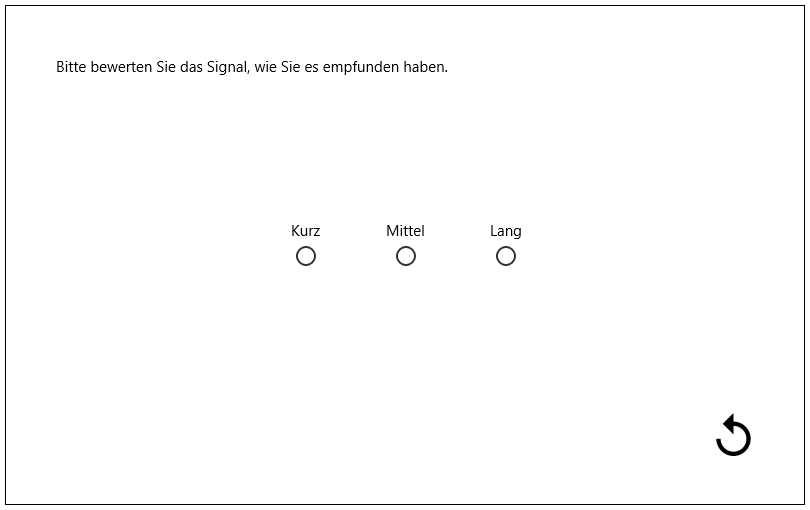
\includegraphics[width=0.65\textwidth]{pics/gui/GrenzenBestimmen.png}
%    \caption{GUI zur Bestimmung der Grenzen}
%    \label{fig:GrenzenBestimmen}
%\end{figure}

Nachdem der Proband die Angaben zur Person beantwortet hat, erscheint ein Benachrichtigungsfenster, indem Informationen {\"u}ber den die aktuelle Phase erkl{\"a}rt wird. 
Falls der Proband zu einem Zeipunkt Fragen haben sollte, werden diese durch den Aufseher beantwortet.
F{\"u}r die Bestimmung der Grenzen wurden 10 Signale erzeugt, die gleichverteilt sind. 
Mithilfe einer Zufallsfunktion werden diese Signale zuf{\"a}llig ausgew{\"a}hlt und in dieser Reihefolge abgespielt. 
Der Proband soll f{\"u}r jeden der 10 Signalen einen der Signaltypen \textit{Kurz}, \textit{Mittel} oder \textit{Lang} zuordnen. 
Dabei habe man die im Entwurf besprochenen Sonderf{\"a}lle {\"u}berpr{\"u}ft und bei erfolgreicher Bildung der Grenzen ist man in die n{\"a}chste Phase {\"u}bergegangen.
%Als alle 10 Signale bewertet wurden, hat man {\"u}berpr{\"u}ft, ob der Kleinste Wert von 100ms Kurz und der gr{\"o}{\ss}te Wert von 1000ms Lang gewesen ist. 

Wenn die Bestimmung der Grenzen nicht erolgreich gewesen ist, wird der Benutzer gebeten die gleiche zuf{\"a}llige Reihenfolge erneut zu bewerten. 

Sollte ein Proband den Replay-Button dr{\"u}cken, wird das letzte Signal erneut abgespielt.

F{\"u}r die GUI \autoref{fig:GrenzenBestimmen} hat man sich auf das wesentliche beschr{\"a}nkt. Die Anweisung an den Benutzer war immer die selbe, daher hat man nur den gleichen Text dargestelllt. Als Antwortm{\"o}glichkeiten des Signals wurde f{\"u}r jeden Sognaltyp je ein Radio-Button erstellt. 
In den Phasen, in denen ein Signal abgespielt wurde, wurde der Replay-Button immer an der gleichen feste Position plaziert. 

Der Ablauf einer Bewertung wird im folgenden beschrieben. Nach der Best{\"a}tigung des Benachrichtigungsfenster wurden im Hintergrund die 10 Signale in zuf{\"a}lliger Reihenfolge ausgew{\"a}hlt. Darauf wurde das erste Signal {\"u}ber BLE an das Wearable gesendet. Das Wearable hat dieses Signal empfangen, ausgewertet und hat die Informationen als Vibration abgespielt. Das was der Benutzer dadurch empfunden hat wurde {\"u}ber den PC mittels der Maus bewertet. Nach einer Bewertung gab es keine M{\"o}glichkeit die Bewertung eines vorherigen Signals erneut anzupassen. Nachdem das Signal vom Probanden bewertet wurde, wurde der Maus-Cursor durch dem Programm an eine Anfangsposition gesetzt, damit der Benutzer nicht unabsichtlich doppelt auf ein Radio-Button dr{\"u}cken konnte. Um dem Probanden zu signalisieren, dass er die Checkbox gedr{\"u}ckt hat, hat man die Check-Box einen Augenblick visuell markiert gelassen, nachdem man den Maus-Cursor neu positioniert hat. Mit der Neupositionierung der Maus hat man erreicht, dass man immer den gleichen Weg hatte um die Checkboxen zu erreichen, aber man hatte auch nach mehreren Fragen die Maus anheben weiter nach oben legen m{\"u}ssen, denn man hat schon das Ende der Tischkannte erreicht. Nach einer Bewertung wurde die vorherige Auswahl entfernt und man hat das n{\"a}chste Signal {\"u}bertragen.

\section {Ausf{\"u}hren des Algorithmus}

%\begin{figure}[htbp] 
%	\centering
%	\begin{minipage}[t]{0.65\textwidth}
%		\includegraphics[width=\textwidth]{pics/gui/{Algorithmus1}.png}
%	\end{minipage}
%	\begin{minipage}[t]{0.65\textwidth}
%		\includegraphics[width=\textwidth]{pics/gui/{Algorithmus2Emotion}.png}
%	\end{minipage}
%	\caption{GUI des Algorithmus (links) und der Bewertung der Stimmung (rechts)}
%	\label{fig:AlgorithmusBild}
%\end{figure}

F{\"u}r den Algorithmus habe man sich mehrere Klassen erzeugt. 
Die Klasse \textbf{DNA} beinhaltet ein Signal und Hilfsfunktionen, die eine Rekombination und eine Muatation von zwei Signalen erzeugen.
In der Klasse \textbf{Population} hat man eine Liste aus 30 Elementen, von einer Klasse \textbf{DNA} erstellt, dabei sind beinhalten die ersten 10 DNA-Objekte Signale, die den Signaltypen \textit{Kurz} haben. F{\"u}r die nachfolgenden DNA-Objekte gilt das selbe nur mit \textit{Mittel} gefolgt von \textit{Lang}. 
Bei der Erzeugung der Signale habe man mittels einer Zufallsfunktion sich Signale mit einer zuf{\"a}lligen St{\"a}rke und einer zuf{\"a}lligen L{\"a}nge zwischen den Grenzen des jeweiligen Signaltypens erstellt. Beim ersten Aufruf der Klasse \textit{Population} habe man die Grenzen der Signaltypen ebenfalls als ein Signal erzeugt und in der Liste hinzugef{\"u}gt.

F{\"u}r die Grafische Benutzeroberfl{\"a}che \autoref{fig:AlgorithmusBild} hat man sich f{\"u}r die drei folgenden Fragen entschieden:
\begin{itemize}
\item Was f{\"u}r einen Signaltypen haben Sie erkannt?
\item Wie gut haben Sie das Signal erkannt?
\item Wie empfanden Sie die St{\"a}rke des Signals?
\end{itemize}

Es ist bis auf die Anzahl der Fragen genau das gleiche Prozedere gewesen. Es wurde zuerst ein Erkl{\"a}rungsfenster dargestellt, so dass der Benutzer wei{\ss}, was in dieser Phase von Ihm erwartet wird. 
Dabei wird im Hintergrund wie gerade erw{\"a}hnt eine Population erzeugt. Diese Population wird DNA f{\"u}r DNA abgearbeitet. Dabei wird f{\"u}r jede DNA enthaltene Signal {\"u}ber BLE an das Wearable gesendet und die Information in Vibration umgewandelt. Dabei hat der Benutzer die drei Fragen zu dem Signal beantworten sollen. 
Es musste die komplette Population bewertet werden, es wurde keine DNA erneut bewertet. Man habe dabei zuf{\"a}llig eine DNA aus der Population gew{\"a}hlt, die bewertet werden sollte.

Die erste Frage diente nur dazu um in der sp{\"a}teren Auswertung herauszufinden, was der Benutzer im Vergleich zum Programm erkannt hat. 
Die zweite Frage wurde als eigentlicher Fitnesswert gespeichert. Die Repr{\"a}sentation der Frage ist in der Tabelle \autoref{} TODO zu sehen.
Die St{\"a}rke wurde direkt nach der Beantwortung aller drei Fragen nach dem Zustandsdiagramm ver{\"a}ndert.

Die Informationen der St{\"a}rke und des Fitnesswerts habe man in der Klasse \textit{Signal} noch mitgespiechert.

Nachdem eine Population komplett berechnet wurde, habe man den Generations-z{\"a}hler um eins erh{\"o}ht, die bisherigen Informationen in der externen Datei gespeichert und eine neue Population aus den Werten erzeugt.

%Die Erzeugung ist dabei so vonstatten gegangen:...
\paragraph{Selektion}
F{\"u}r jeden Signaltypen legt man einen Pool aus DNA-Objekten an, dessen Signale den jeweiligen Signaltypen besitzen.
Mithilfe der Formel X (im Entwurf) berechnet man die Anzahl, wie oft ein DNA-Objekt in das jeweilige Pool hinzugef{\"u}gt werden soll. Man legt genausoviele DNA-Objekte, wie berechnet in das Pool. 
Im Durchschnitt besitzt ein Pool nach dem hinzuf{\"u}gen der H{\"a}ufigkeit aller DNA-Objekte in etwa bis zu 1000 Elemente.
%Im Durchschnitt hat man nach dem hinzug{\"u}gen aller DNA-Objekte in etwa 1000 Elemente in einem der Pools. 
Die Selektion erfolgt per Zufallsprinzip, dabei w{\"a}hlt man zwei zuf{\"a}llige DNA-Objekte aus einem Pool. Diese beiden DNA-Objekte werden auch als \textit{Eltern} bezeichnet. Die beiden Eltern erzeugen nun durch Ausf{\"u}hrung der \textit{Rekombination} und \textit{Mutation} einen Nachkommen f{\"u}r die Population der n{\"a}chsten Generation. Dabei wird es so lange wiederholt, bis man genauso viele Individuen wie aus der Population der vorherigen Generation vorhanden waren.

\paragraph{Rekombination}
In der Rekombination verwendet man die Eltern, greift man auf die jeweiligen Signale zu und verwendet die beiden Attribute L{\"a}nge und St{\"a}rke. 
F{\"u}r die beide Attribute bildet man den Mittelwert, die ganzzahlig abgerundet werden.
Diese Attribute bilden werden f{\"u}r die Erzeugung des neuen Individuums verwendet.

\paragraph{Mutation und Termination}
Es existiert eine f{\"u}nf Prozentige Chance, dass das neu erzeugte Individuum durch ein zuf{\"a}llig generiertes Signal ersetzt wird. 

Nachdem die vierte Generation erzeugt wurde, wird der Algorithmus terminiert. Aus der zuletzt erzeugten Population werden f{\"u}r die L{\"a}nge und St{\"a}rke die Grenzen der drei Signaltypen bestimmt. Die Grenzen dienen als Eingabe f{\"u}r die Erzeugung der personalisierten Muster. 


%Nachdem die vierte Generation erzeugt wurde, bestimmt man an der neu erzeugten Population den Mittelwert der Grenzen f{\"u}r die St{\"a}rke und L{\"a}nge der Signaltypen \textit{Kurz}, \textit{Mittel} und \textit{Lang}. 
Die gerade bestimmten Mittelwerte bilden die personalisierten Werte, die f{\"u}r die Mustererkennung verwendet werden. 
%Der Algorithmus wird nach der vierten Iteration terminiert und es wird mit der \textit{Erkennung der Muster} fortgefahren.
%Sobald die vierte Generation erreicht worden ist, wird die zuletzt erzeugte Population verwendet. Dabei verwendet man bestimmt man f{\"u}r jeden Signaltypen 

\section {Muster Erkennung}

%\begin{figure}[htbp] 
%	\centering
%	\begin{minipage}[t]{0.65\textwidth}
%		\includegraphics[width=\textwidth]{pics/gui/{Muster1}.png}
%	\end{minipage}
%	\begin{minipage}[t]{0.65\textwidth}
%		\includegraphics[width=\textwidth]{pics/gui/{Muster2}.png}
%	\end{minipage}
%	\caption{GUI des Musters ohne Eingabe (links) und (rechts) nach der Eingabe}
%	\label{fig:MusterBild}
%\end{figure}

F{\"u}r die Erzeugung der Muster hat man die Grenzen mit {\"u}bergeben m{\"u}ssen, denn in der Klasse \textit{Muster} wird der personalisierte Wert bestimmt, dies geschieht, indem man Mittelwert der Grenzen berechnet. 
Im Vorfeld hat man drei Typen von Mustern erstellt. F{\"u}r jeden Muster-Typen hat man 15 Muster angelegt. 
F{\"u}r jeden Muster-Typen habe man zwei Listen angelegt, dabei wurden alle 15 Muster hineingelegt mit dem einzigen Unterschied, dass in der einen Liste die Muster mit personalisierten Werten und in der anderen Liste die Muster mit den generischen Werten vorhanden sind.
Die generischen Werte f{\"u}r \textit{Kurz}, \textit{Mittel} und \textit{Lang} sind 200ms, 400ms und 800ms gewesen, alle Signale wurden mit dem Wert \textit{Stark} f{\"u}r die St{\"a}rke inizialisiert.
Als n{\"a}chstes wurden die Listen in zuf{\"a}lliger Reihenfolge geordnet. 
Die Initialisierung hat einige Sekunden in Anspruch genommen, da man jedoch vermeiden wollte, dass zur Laufzeit ein Fehler dadurch passieren w{\"u}rde. Diese Wartezeit hat man akzeptiert und dem Probanden darauf Aufmerksam gemacht.

%Um die Muster zu erzeugen hat man im Vorfeld erst einmal Muster-Objekte erzeugt. 
%Die Muster wurden im Vorfeld f{\"u}r alle Benutzer einmalig festgelegt.
%Es gab drei verschiedene Arten, einmal Objekte mit drei Signalen und zwei Pausen, vier Signalen und drei Pausen und f{\"u}nf Signalen und vier Pausen. 
%Man habe f{\"u}r jeden Muster-Typen zwei Listen erstellt und alle Objekte des Muster-Typens in die zwei Listen kopiert, dabei war die erste Liste mit personalisierten Mustern und die andere Liste mit generischen Mustern  
%Diese Objekte hat man in sechs verschiedene Listen gepackt. Dabei habe man drei H{\"u}llen von Mustern gehabt, die drei, vier und f{\"u}nf Signale mit dementsprechenden Pausen ergeugt hatte. Man hat jeweils einen H{\"u}llen-Typen f{\"u}r 2 Listen verwendet. 
%F{\"u}r die beiden Listen mit den dreier Muster H{\"u}llen werden jetzt die Werte auf die personalisierten und vorgegebenen Werte gespeichert. Dies passiert auch mit den vierer und f{\"u}nfer Muster Listen.
%Anschlie{\ss}end werden die schon in einer zuf{\"a}lligen Reihenfolge in der Liste gespeichert. 
%Dies hat zu Beginn einige Sekunden in Anspruch genommen, aber man habe lieber einmalig einige Sekunden warten m{\"u}ssen anstatt w{\"a}hrend man die Muster abspielen w{\"u}rde.
%Dies k{\"o}nnte einerseits fehleranf{\"a}lliger sein und in der jetzigen Variante werden w{\"a}hrend des Bewertung nur noch die Eingabedaten des Benutzers abgespeichert.

Die Muster wurden abwechselnd zwischen den personalisierten und generischen Muster an das Wearable gesendet, dabei hat man die Muster in der Reiehenfolge von den kleinsten bis zum gr{\"o}{\ss}ten Muster-Typen abgespielt. 
Die Probanden hatten die Aufgabe die Reihenfolge der Signaltypen eines Muster anzugeben.
F{\"u}r die GUI \autoref{fig:MusterBild} TODO hat man nur die Bedienelemente anzeigen lassen, die aktuell ben{\"o}tigt waren, man habe n{\"a}mlich f{\"u}r jeden Signaltypen einen Button gehabt. Durch dr{\"u}cken auf einen dieser Buttons ist der Signaltyp als Eingabe erfolgt und es wurden die Eingaben visuell dargestellt.
Der Proband hat genau die Anzahl an Signalen einzugeben gehabt, wie auch das Muster lang war, es verschwanden die drei Signal-Eingabe-Buttons und zum vorschein kam ein Best{\"a}tigungsbutton. Erst als dieser Button gedr{\"u}ckt wurde, wurde das n{\"a}chste Muster abgespielt und der Button verschwand und die anderen kamen zum vorschein. 
Anhand einem \textit{Clear}-Button hat man die komplette Eingabe entfernen k{\"o}nnen um diese bei Fehlern erneut bewerten zu k{\"o}nnen.
F{\"u}r jedes Muster habe man die M{\"o}glichkeit gehabt, das Muster erneut abzuspielen.  
Bei einem Wechsel der Mustertypen wurde ein Signal vorher dem Probanden {\"u}ber ein Benachrichtigungsfenster darauf aufmerksam gemacht.

W{\"a}hrend des Ablauf der Erkennung der Muster wurden noch die Zeit, die ben{\"o}tigt wurde um ein Muster zu bewerten gespeichert. 



\begin{figure}[htbp] 
	\centering
	\begin{minipage}[t]{0.95\textwidth}
		\includegraphics[width=\textwidth]{pics/gui/{AngabenZurPerson1}.png}
	\end{minipage}
	\begin{minipage}[t]{0.95\textwidth}
		\includegraphics[width=\textwidth]{pics/gui/{AngabenZurPerson2}.png}
	\end{minipage}
	\caption{GUI f{\"u}r die Befragung zu den Angaben zur Person}
	\label{fig:AngabenZurPerson}
\end{figure}

\begin{figure}
	\centering
    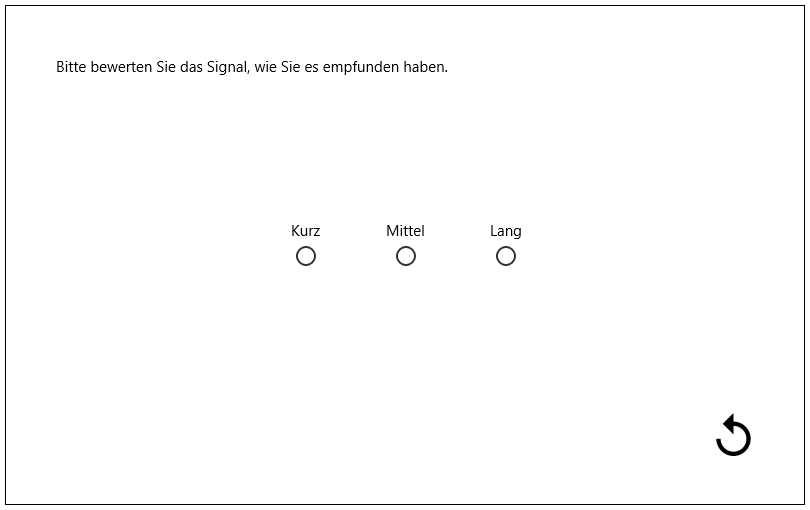
\includegraphics[width=0.95\textwidth]{pics/gui/GrenzenBestimmen.png}
    \caption{GUI zur Bestimmung der Grenzen}
    \label{fig:GrenzenBestimmen}
\end{figure}

\begin{figure}[htbp] 
	\centering
	\begin{minipage}[t]{0.95\textwidth}
		\includegraphics[width=\textwidth]{pics/gui/{Algorithmus1}.png}
	\end{minipage}
	\begin{minipage}[t]{0.95\textwidth}
		\includegraphics[width=\textwidth]{pics/gui/{Algorithmus2Emotion}.png}
	\end{minipage}
	\caption{GUI des Algorithmus (links) und der Bewertung der Stimmung (rechts)}
	\label{fig:AlgorithmusBild}
\end{figure}


\begin{figure}[htbp] 
	\centering
	\begin{minipage}[t]{0.95\textwidth}
		\includegraphics[width=\textwidth]{pics/gui/{Muster1}.png}
	\end{minipage}
	\begin{minipage}[t]{0.95\textwidth}
		\includegraphics[width=\textwidth]{pics/gui/{Muster2}.png}
	\end{minipage}
	\caption{GUI des Musters ohne Eingabe (links) und (rechts) nach der Eingabe}
	\label{fig:MusterBild}
\end{figure}




%Nachdem der Proband genau  die L{\"a}nge des Muster war eingegeben hat, erschien ein Best{\"a}tigungsbutton. 
%Erst dann erschien ein Best{\"a}tigungsbutton, mit dem man die Eingabe best{\"a}tigen konnte. Es gab noch einen L{\"o}schen Button, 
%Das Muster wurde wie die Signale zuvor auch {\"u}ber das Wearable abgespielt dabei , hat man dem Probanden darum gebeten, die einzelnen Signale des Musters anzugeben. 

%Der Proband sollte die M{\"o}glichkeit besitzen nur die Anzahl der Signale eingeben zu k{\"o}nnen, die ein Muster auch besitzt. 


%F{\"u}r jeden Signaltypen hat man einen Button mit dem Anfangsbuchstaben des Typens positioniert. 
%Um die Signaltypen ausw{\"a}hlen zu k{\"o}nnen, hat man f{\"u}r jeden Signaltypen einen Button erstellt. Die Buttons wurden mit dem Anfangsbuchstaben des Signaltypens beschriftet. 

%Dabei hat man die GUI so entworfen, dass man nur das machen konnte, was erlaubt gewesen ist.
%W{\"a}hrend ein Signal abgespielt wurde, hat man die Signal



%\paragraph {1. Aufnahme der Personalien}
%Der erste Schritt bestand darin, den Probanden den Personalien zu fragen. 

%\paragraph {2. Bestimmung der Grenzen durch Bewertung durch den Nutzer}
%\paragraph {3. Ausf{\"u}hren des Algorithmus}
%\paragraph {4. Muster Erkennung} 

%Das Signal ist ein wichtiger Bestandteil meines Programm. 
%Ein Signal beinhaltet die Signall{\"a}nge, die in Millisekunden gespeichert wird, und eine Signalst{\"a}rke, die in 5 St{\"a}rkestufen eingeteilt ist. 



%Ich habe meinen Evolution{\"a}ren Algorithmus so angepasst, dass bei mir ein Induviduum ein Signal ist. 
%Ich habe dem Benutzer das Signal mit dem Wearable abspielen lassen und im Anschluss Fragen beantworten lassen. 
%Er sollte bewerten wie gut er das Signal erkannt hat. Die Bewertung vom Benutzer war entscheidend um nach der kompletten Bewertung der Population 

% -----------------------------------------------------------------------

%\paragraph {1. Aufnahme der Personalien}


%Um in der Evaluierung m{\"o}gliche Erkentnisse zwischen bestimmten Benutzergruppen herausfinden zu k{\"o}nnen, hat man dem Benutzer Eine Reihe von Fragen gestellt, die im Bild XXXX zu sehen sind.
%Diese Daten wurden anonymisiert gespeichert. 

%\paragraph {2. Bestimmung der Grenzen durch Bewertung durch den Nutzer}


%\paragraph {3. Ausf{\"u}hren des Algorithmus}


%\paragraph {4. Muster Erkennung} 

%MUSTER BILD

